
\documentclass[preprint,12pt]{elsarticle}

\usepackage[spanish]{babel}
\usepackage{amssymb}
\usepackage{graphicx}
\usepackage{lineno}
\usepackage[utf8]{inputenc}
\usepackage{url}
\usepackage{natbib}

\begin{document}
	
	\begin{frontmatter}

		\title{\huge  Laboratorio 03: Creando un Reporte Interactivo en Power BI	 }
		\author{	Tarqui Montalico,Risther(2017057469)}
		
		





\end{frontmatter}

%%INICIO Resumen
\section{Objetivo}
	
	Comprender el funcionamiento de Qlik realizando un ejercicio con intrucciones precisas.
%%FIN Resumen


%%INICIO Introducción
\section{Desarrollo}

	\begin{itemize}
			TARE 01: Conectar con power BI a datos \\
		
		 		\\ 1. Abrir SQL Server Management Studio, y conectar a la instancia de base de datos (local) utilizando
		 		autenticación de Windows.
		 		 \\ 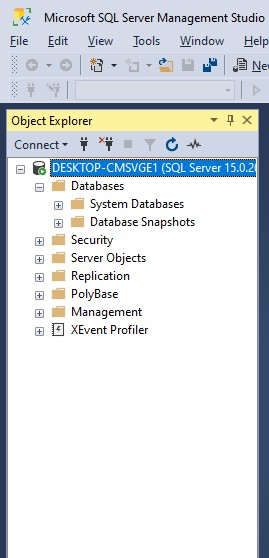
\includegraphics[width=4cm]{./IMAGENES/1.1.1} \\
		 		\\ 2. En el menú Archivo (File), en el submenu Abrir (Open), hacer click en Project/Solution, y buscar el archivo
		 		Project.ssmssln.
		 		\\ 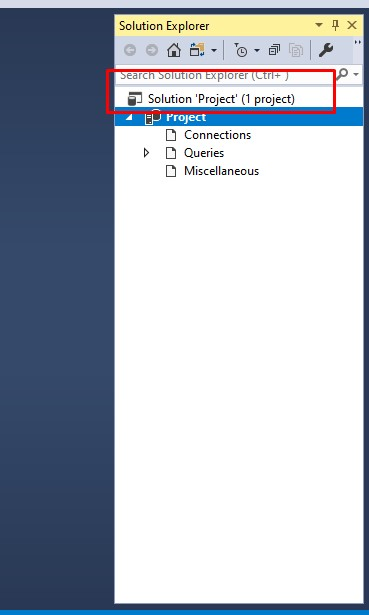
\includegraphics[width=4cm]{./IMAGENES/1.1.2} \\
		 		\\ 3. En el Explorador de Soluciones, expandir Consultas (Queries), y luego hacer doble click en el archivo Lab
		 		Exercise 1.sql.
		 	\\ 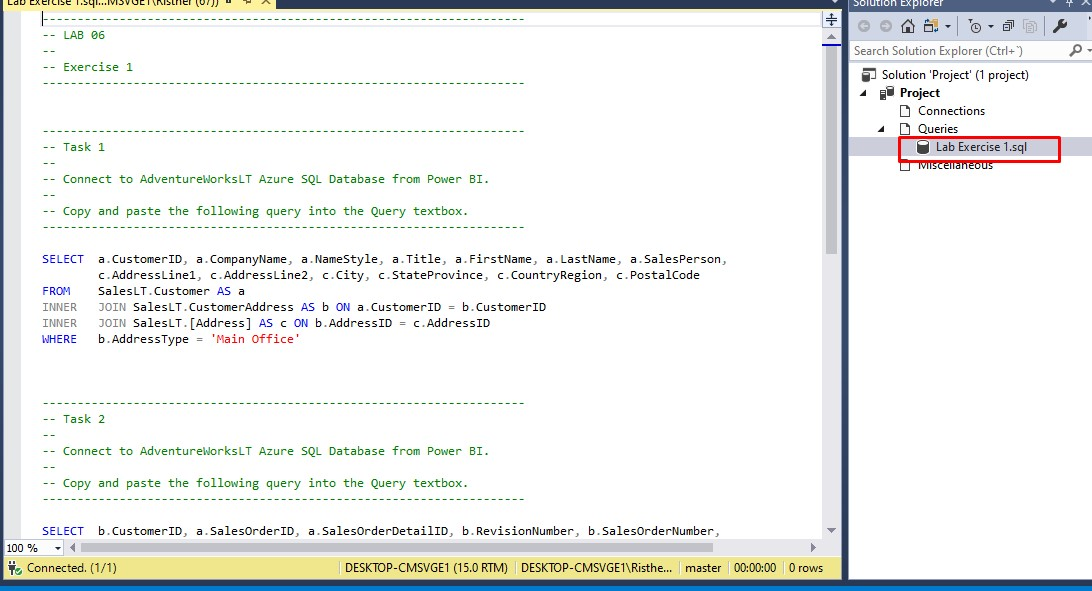
\includegraphics[width=10cm]{./IMAGENES/1.1.3} \\
		 		\\ 4. Abrir Power BI Desktop.
		 	\\ \includegraphics[width=10cm]{./IMAGENES/1.1.4} \\
		 		\\ 5. En la ventana Power BI Desktop, hacer click en Obtener Data (Get Data).
		 	\\ 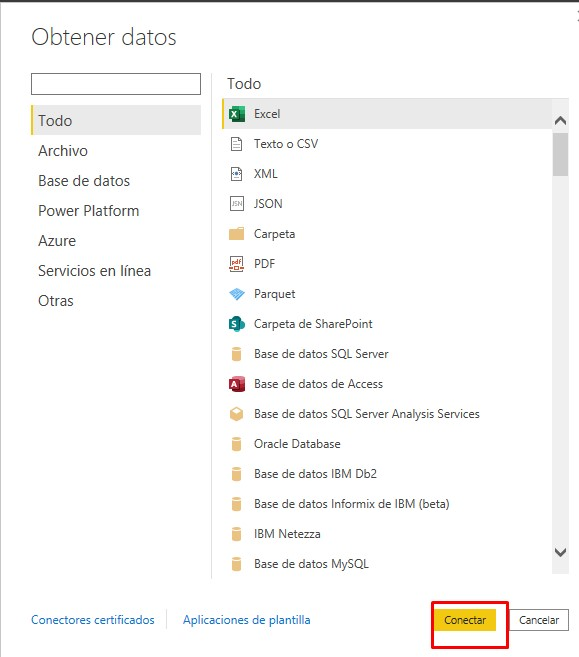
\includegraphics[width=10cm]{./IMAGENES/1.1.5} \\
		 		\\ 6. En el cuadro Obtener Datos, click base de datos Microsoft SQL, y entonces click en Conectar
		 		\\ 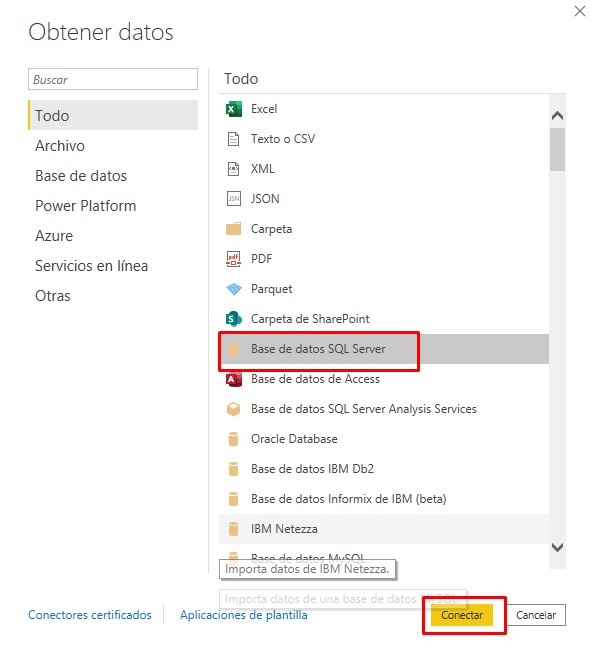
\includegraphics[width=10cm]{./IMAGENES/1.1.6} \\
		 		\\ 7. En la ventana base de datos Server database, En Servidor, escribir (local).
		 	\\ \includegraphics[width=10cm]{./IMAGENES/1.1.7} \\
		 		\\ 8. En Base de Datos (opcional), tipear AdventureWorksLT.
		 		\\ 9. Expandir el cuadro Opciones Avanzadas. Copiar el script Task 1 del archivo \\ Lab Exercise 1.sql. y pegar
		 	\\ 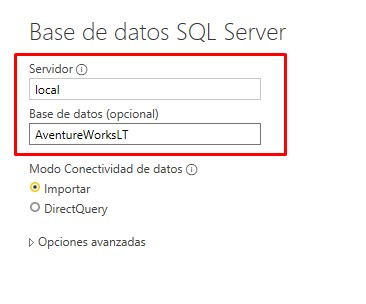
\includegraphics[width=10cm]{./IMAGENES/1.1.8} \\
		 		\\ la consulta en Power BI, en el cuadro sentencia SQL. Luego presionar OK.
		 		\\ 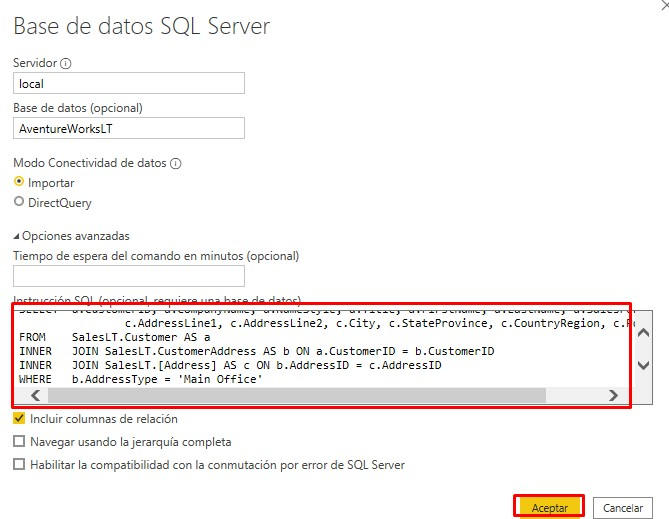
\includegraphics[width=10cm]{./IMAGENES/1.1.9} \\
		 		\\ 10. En la ventana de vista preliminar click en Cargar.
		 		\\ 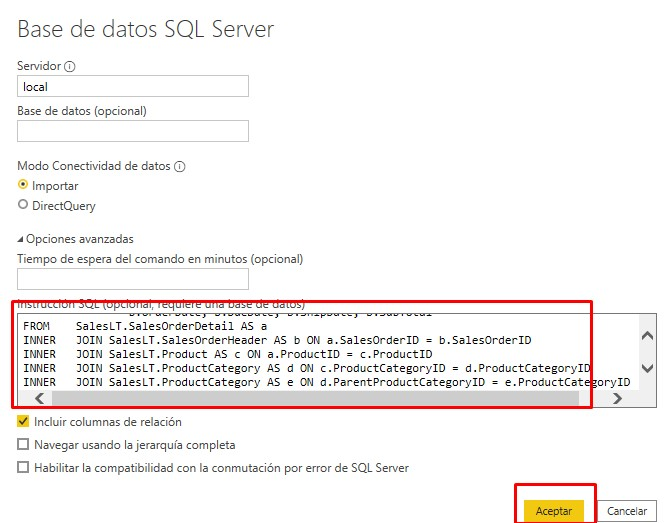
\includegraphics[width=10cm]{./IMAGENES/1.1.10} \\
		 		\\ 11. En Power BI Desktop, click Obtener Datos y luego click en Mas.
		 	
		 		\\ 12. Repetir los pasos del 6 al 10, utilizando el script Task 2.
		 		
		 		\\ 13. De regreso en el reporte. Guardar el archivo como AdventureWorksLT Sales.pbix.
		 	\\ 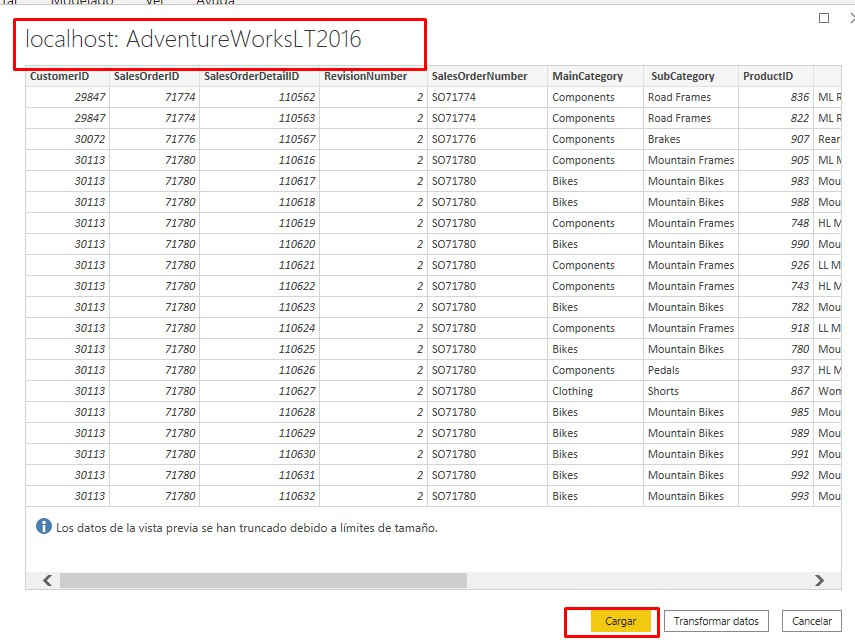
\includegraphics[width=10cm]{./IMAGENES/1.1.11} \\
		 	
		 	
		 		TAREA 02: Graficar ddatos \\ 
		 		\\ 1. En el panel Campos (Fields), click derecho sobre Query1, Renombrar, tipear Customers y presionar Enter.
		 		\\ 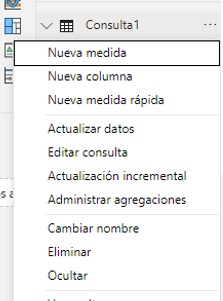
\includegraphics[width=10cm]{./IMAGENES/2.1} \\
		 		\\ 2. Para el Query2, hacer lo mismo del paso 1 y colocar el nombre Sales.
		 		\\ 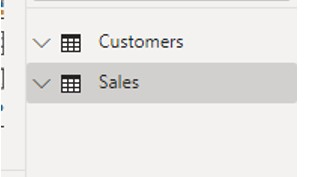
\includegraphics[width=10cm]{./IMAGENES/2.2} \\
		 		\\ 3. Expandir ambas tablas para ver todas las filas.
		 		\\ 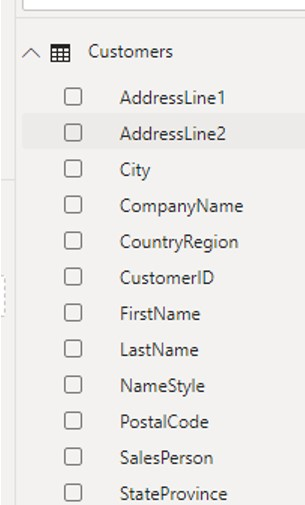
\includegraphics[width=10cm]{./IMAGENES/2.3} \\
		 		\\ 4. En la barra de navegación, click Datos (Data).
		 		Pág. 2
		 		\\ 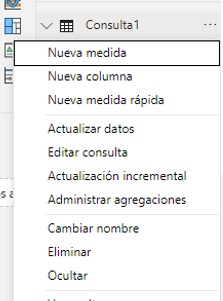
\includegraphics[width=10cm]{./IMAGENES/2.1} \\
		 		\\ 5. In the Fields pane, click the Customers table, if it is not already selected.
		 		\\ 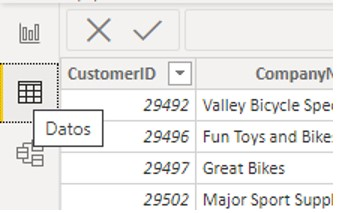
\includegraphics[width=10cm]{./IMAGENES/2.4} \\
		 		\\ 6. Right-click the NameStyle column, and click Delete.
		 		\\ 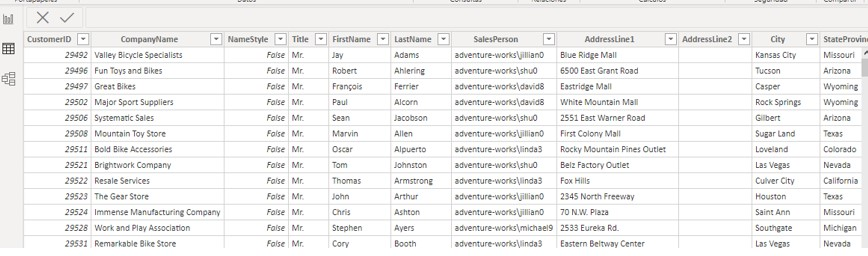
\includegraphics[width=10cm]{./IMAGENES/2.5} \\
		 		\\ 7. In the Delete Column dialog box, click Delete.
		 		\\ 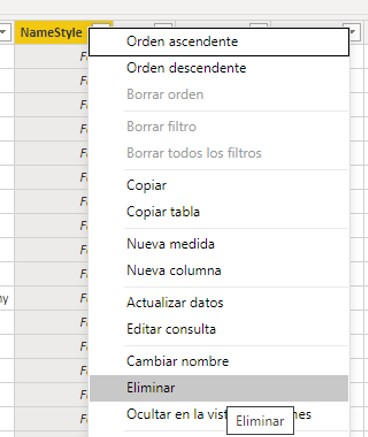
\includegraphics[width=10cm]{./IMAGENES/2.6} \\
		 		\\ 8. Repetir el paso 6 y 7 para la columna SalesPerson.
		 		\\ 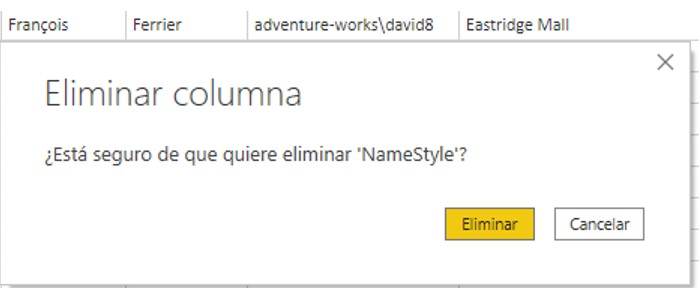
\includegraphics[width=10cm]{./IMAGENES/2.7} \\
		 		\\ 9. Right-click the CustomerID column, and then click Hide in Report View.
		 		\\ 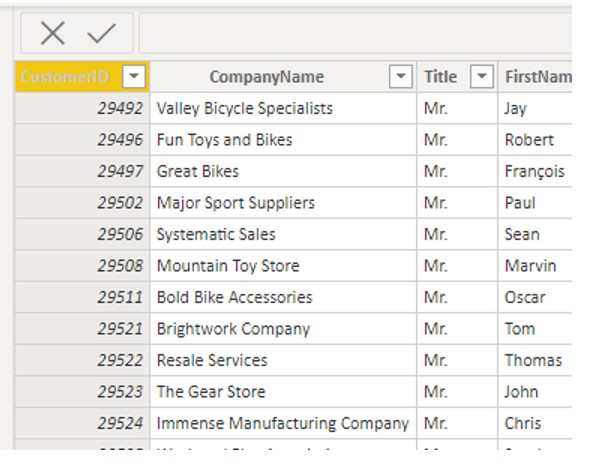
\includegraphics[width=10cm]{./IMAGENES/2.9} \\
		 		\\ 10. Click the AddressLine1 column header.
		 		\\ \includegraphics[width=10cm]{./IMAGENES/2.10} \\
		 		\\ 11. On the Modeling ribbon, in the Properties group, click Data Category: Uncategorized, and then click
		 		Address.
		 		\\ 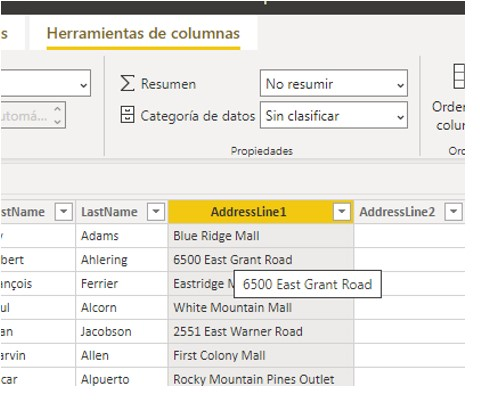
\includegraphics[width=10cm]{./IMAGENES/2.11} \\
		 		\\ 12. Click the City column header.
		 		\\ 13. On the Modeling ribbon, in the Properties group, click Data Category: Uncategorized, and then click City.
		 		\\ 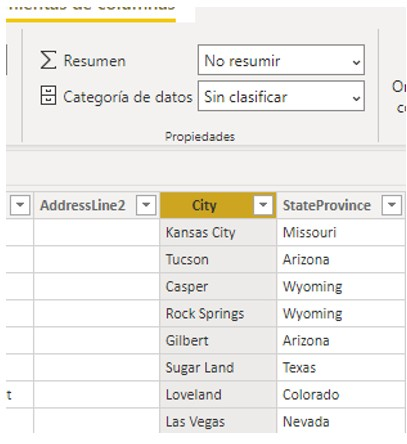
\includegraphics[width=10cm]{./IMAGENES/2.13} \\
		 		\\ 14. Click the StateProvince column header.
		 		\\ \includegraphics[width=10cm]{./IMAGENES/2.14} \\
		 		\\ 15. On the Modeling ribbon, in the Properties group, click Data Category: Uncategorized, and then click State or
		 		Province.
		 		\\ 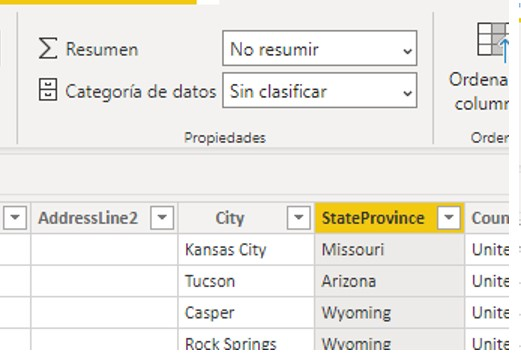
\includegraphics[width=10cm]{./IMAGENES/2.15} \\
		 		\\ 16. Click en el encabezado de columna CountryRegion.
		 		\\ 17. On the Modeling ribbon, in the Properties group, click Data Category: Uncategorized, and then click
		 		Country/Region.
		 		\\ 18. Click en el encabezado de columna PostalCode.
		 		\\ 19. On the Modeling ribbon, in the Properties group, click Data Category: Uncategorized, and then click Postal
		 		Code.
		 		\\ 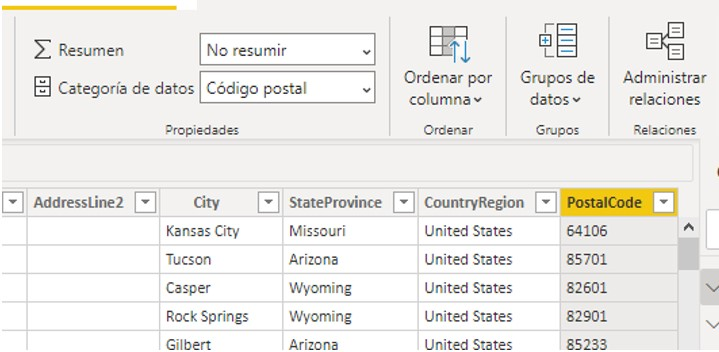
\includegraphics[width=10cm]{./IMAGENES/2.19} \\
		 		\\ 20. On the Modeling ribbon, in the Calculations group, click New Column, and then in the formula bar, type the
		 		following expression and press Enter:
		 		\\ 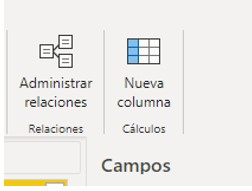
\includegraphics[width=10cm]{./IMAGENES/2.20} \\
		 		\\ 21. In the Fields pane, click Sales.
		 		\\ 22. Right-click the RevisionNumber column, and click Delete.
		 		\\ 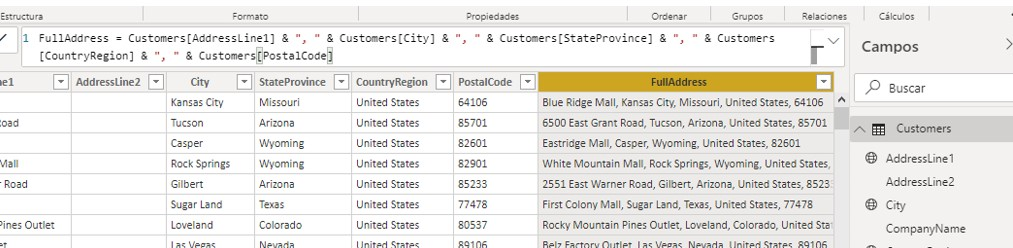
\includegraphics[width=10cm]{./IMAGENES/2.21} \\
		 		\\ 23. In the Delete Column dialog box, click Delete.
		 		\\ 24. Realizar el paso 23 y 34 para la columna SalesOrderNumber.
		 		\\ \includegraphics[width=10cm]{./IMAGENES/2.24} \\
		 		\\ 25. Right-click the CustomerID column, and then click Hide in Report View.
		 		26. Realizar el paso 26 para las columnas SalesOrderID y SalesOrderDetailID.
		 		\\ 27. On the Modeling ribbon, in the Calculations group, click New Column, and then in the formula bar, type the
		 		following expression and press Enter:
		 		\\ 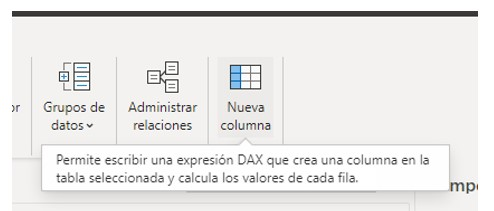
\includegraphics[width=10cm]{./IMAGENES/2.27} \\
		 		\\ 28. Click the LineTotal column header.
		 		\\ 29. On the Modeling ribbon, in the Formatting group, click Format: General, point to Currency, and then click 
		 		English (United States).
		 		\\ 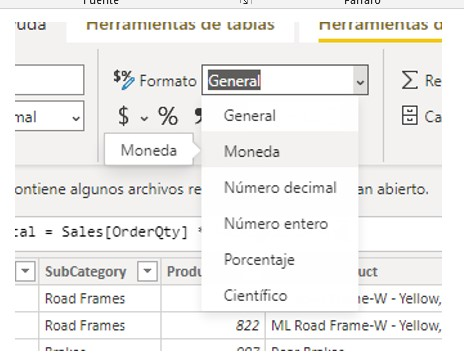
\includegraphics[width=10cm]{./IMAGENES/2.29} \\
		 		\\ 30. On the Modeling ribbon, in the Calculations group, click New Measure, and then in the formula bar, type the
		 		following expression and press Enter.
		 		\\ 31. Click Save, and then leave Power BI Desktop open for the next task.
		 		
		 		on, click Reduce Rows, click Remove Rows, and then click Remove Bottom Rows.
		 		\\ 13. In the Remove Bottom Rows dialog box, in the Number of rows box, type 26, and then click OK.
		 		\\ 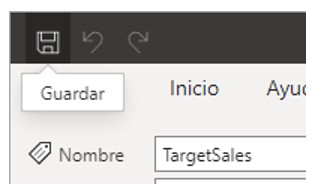
\includegraphics[width=10cm]{./IMAGENES/2.30} \\
		 		
		 		
		 		\\ Tarea 3: Combinar Data \\ 
		 		\\ \\ 1. In File Explorer, and then open the States.xlsx file.
		 		\\ 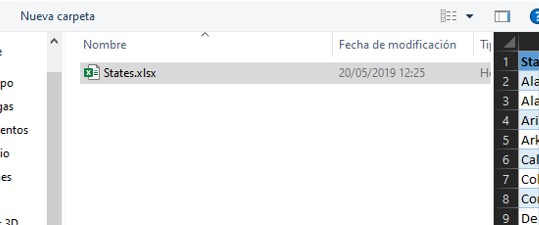
\includegraphics[width=10cm]{./IMAGENES/3.1} \\
		 		\\ 2. In the States worksheet, select all of the values in the two columns, and then press Ctrl+C.
		 		\\ 3. In Power BI Desktop, on the Home ribbon, click Enter Data.
		 		\\ 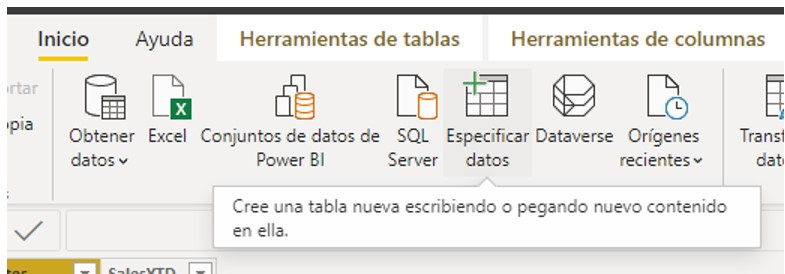
\includegraphics[width=10cm]{./IMAGENES/3.3} \\
		 		\\ 4. In the Create Table dialog box, click in the table, and then press Ctrl+V. Power BI detects that thefirst row is
		 		a column header.
		 		\\ 5. In the Name box, type Sales by State, and then click Load.
		 		\\ 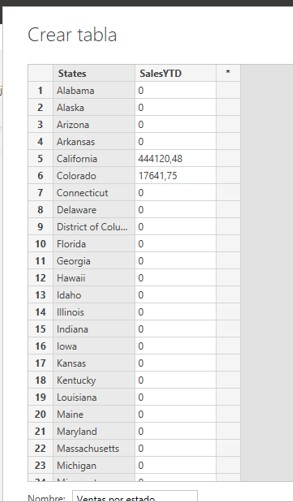
\includegraphics[width=10cm]{./IMAGENES/3.5} \\
		 		\\ 6. On the Home ribbon, click Get Data, and then click Web.
		 		Pág. 3
		 		\\ 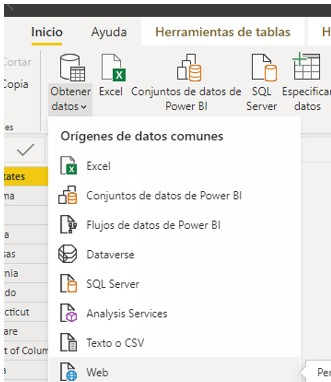
\includegraphics[width=10cm]{./IMAGENES/3.6} \\
		 		\\ 7. In the From Web dialog box, in the URL box, type
		 		\\ \includegraphics[width=10cm]{./IMAGENES/3..7} \\
		 		\\ 8. In the Navigator dialog box, select Codes and abbreviations for U.S. states, territories and other
		 		regions, and then click Load.
		 		\\ 9. In the Fields pane, click Codes and abbreviations for U.S. states, territories and other regions to
		 		display the data. The table has 26 rows at the bottom that are not needed.
		 		\\ 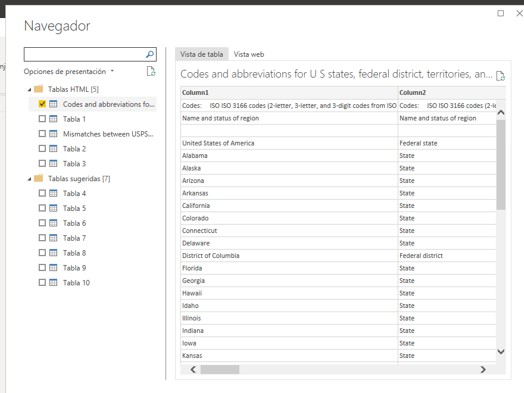
\includegraphics[width=10cm]{./IMAGENES/3.9} \\
		 		\\ 10. On the Home ribbon, in the External Data group, click Edit Queries, then click Edit Queries.
		 		\\ 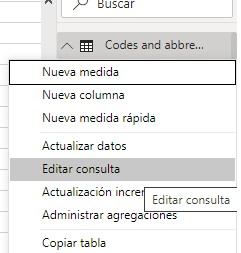
\includegraphics[width=10cm]{./IMAGENES/3.10} \\
		 		\\ 11. In Query Editor, in the Queries pane, click Codes and abbreviations for U.S. states, territories and other
		 		regions.
		 		\\ 12. On the Home ribbon, click Reduce Rows, click Remove Rows, and then click Remove Bottom Rows
		 		\\ 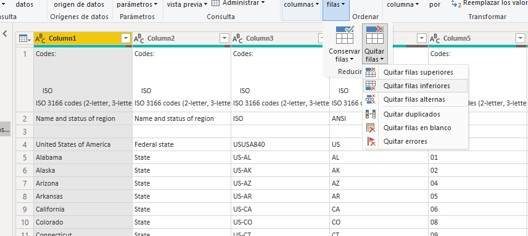
\includegraphics[width=10cm]{./IMAGENES/3.12} \\
		 		\\ 14. Click the ANSI2 column header, and then hold down the Ctrl key while selecting all of the columns to the
		 		right. This selects multiple rows.
		 		\\ 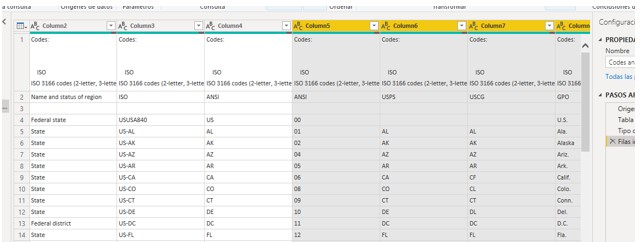
\includegraphics[width=10cm]{./IMAGENES/3.14} \\
		 		\\ 15. Still holding down Ctrl, click the Name and status of region2 and Header columns to include this in the
		 		selection.
		 		\\ 16. On the Home ribbon, click Manage Columns, click Remove Columns, and then click Remove Columns.
		 		\\ 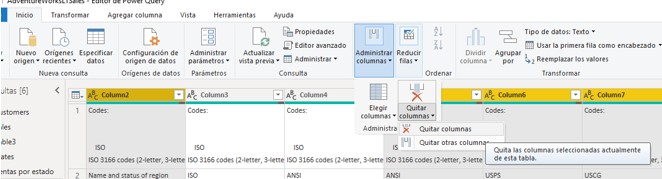
\includegraphics[width=10cm]{./IMAGENES/3.16} \\
		 		\\ 17. In the Query Settings pane, under Properties, in the Name box, type States with Codes, and then press
		 		Enter.
		 		\\ 18. On the Home ribbon, in the Transform group, click Use First Row as Headers.
		 		\\ 19. Right-click the United States of America column header, click Rename, type State Name, and then press
		 		Enter.
		 		\\ 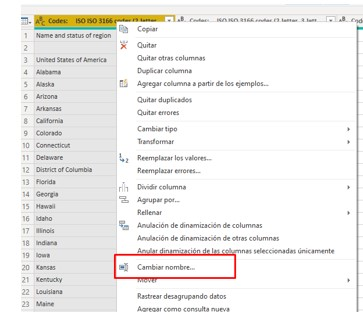
\includegraphics[width=10cm]{./IMAGENES/3.19} \\
		 		\\ 20. Right-click the US USA 840 column header, click Rename, type State Code Long, and then press Enter.
		 		\\ 21. Right-click the US column header, click Rename, type State Code Short, and then press Enter.
		 		\\ 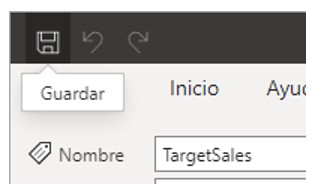
\includegraphics[width=10cm]{./IMAGENES/2.30} \\
		 		\\ 22. In the Queries pane, click Sales by State.
		 		\\ 23. On the Home ribbon, click Combine, and then click Merge Queries.
		 		\\ 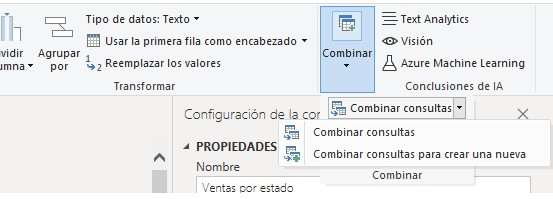
\includegraphics[width=10cm]{./IMAGENES/3.23} \\
		 		\\ 24. In the Merge dialog box, in the Sales by State table, click the States column.
		 		\\ 25. In the list, click States with Codes, click the State Name column, and then click OK. The new column is
		 		added to the table and contains the merged States with Codes table.
		 		\\ 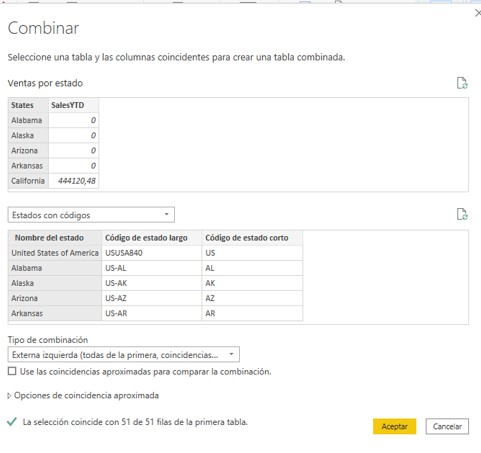
\includegraphics[width=10cm]{./IMAGENES/3.25} \\
		 		\\ 26. In the column header, click the Expand icon, clear (Select All Columns), select State Code Short,
		 		and then click OK. The column now shows just the state codes.
		 		\\ 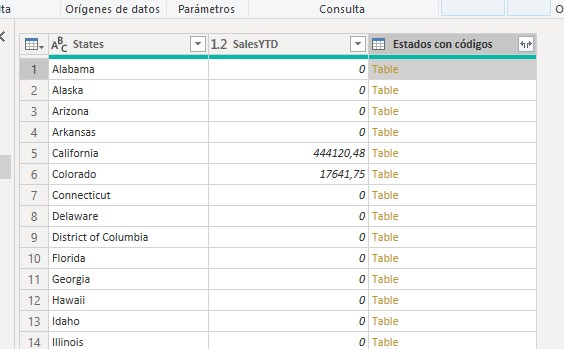
\includegraphics[width=10cm]{./IMAGENES/3.26} \\
		 		\\ 27. Right-click the column, click Rename, type State Code, and then press Enter.
		 		\\ 28. On the File menu, click Close  Apply.
		 		\\ 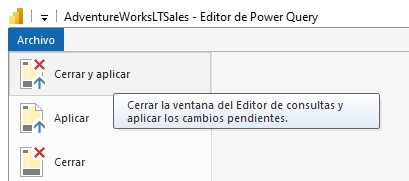
\includegraphics[width=10cm]{./IMAGENES/3.28} \\
		 		\\ 29. In the Fields pane, right-click States with Codes, and then click Hide in Report View.
		 	
		 			\\ 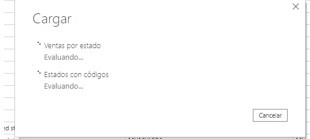
\includegraphics[width=10cm]{./IMAGENES/3.29} \\
		 	
	 
	\end{itemize}
\section
%%FIN Introducción
\section{Ejercicio 2: Construyendo Reportes en Power BI}

	\begin{itemize}
			Tarea 1: Crear un Gráfico\\ 
			\\ 1. En Power BI Desktop, en la barra derecha de navegación, hacer click en Reporte (Report).
				\\ 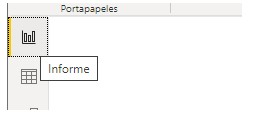
\includegraphics[width=10cm]{./IMAGENES/4.1} \\
			\\ \\ \\ \\ 2. En el panel de Visualizaciones (Visualizations), hacer click en Gauge.
				\\ \includegraphics[width=10cm]{./IMAGENES/4.2} \\
			3. Arrastar el campo LineTotal de la table Sales a la propiedad Valor (Value) del objeto gauge.
				\\ \includegraphics[width=10cm]{./IMAGENES/4.3} \\
			4. Arrastrar la medida TargetSales de la table Sales a la propiedad Valor destino (Target value) del objeto
			gauge.
				\\ \includegraphics[width=10cm]{./IMAGENES/4.4} \\
			5. Hacer click Format, exppandir Gauge axis, and then in the Max box, type 146000.
			\\ 6. Expandir Titulo (Title), en el cuadro Texto de Titulo (Title Text), tipear Meta de Ventas (Target Sales), y
			luego hacer click en Center.
				\\ \includegraphics[width=10cm]{./IMAGENES/4.6} \\
			\\ 7. Click the report canvas, and then drag the CompanyName field from the Customers table onto the report.
			Power BI automatically creates a table.
			\\ 8. Arrastar the LineTotal field from the Sales table onto the report.
		\\ 	9. Make sure that the table has focus, and then in the Visualizations pane, click Pie chart.
			\\ \includegraphics[width=10cm]{./IMAGENES/4.9} \\
			\\ 10. Expand the chart to make all of the company names visible by using the resizer handles on the edge
			of the chart.
				\\ \includegraphics[width=10cm]{./IMAGENES/4.10} \\
			\\ 11. With the focus still on the pie chart, click Format, and then expand Title.
				\\ \includegraphics[width=10cm]{./IMAGENES/4.11} \\
			\\ 12. In the Title Text box, type Top Selling Customers, and then click Center.
			\\ 13. Arrastar el campo MainCategory de la tabla Sales table onto the report canvas. Power BI creates a table.
				\\ \includegraphics[width=10cm]{./IMAGENES/4.13} \\
			\\ 14. Arrastar el campo OrderQty dentro de la tabla.
			\\ 15. In the Visualizations pane, click Stacked bar chart.
			\\ 16. In the Visualizations pane, click Fields.
		\\ 	17. Drag the OrderQty field onto the Color saturation property. Notice that the colors change.
			\\ 18. In the Visualizations pane, click Analytics, expand Constant Line, and then click Add.
			\\ 19. In the Value box, type 500.
			\\ 20. Change Color to red, toggle Data label to On, and then change the color to red.
			\\ 21. In the Visualizations pane, click Format, and expand Title.
			\\ 22. In the Title Text box, type Orders by Main Category, and then click Center.
			\\ 23. Click the report canvas to give it focus, and then in the Visualizations pane, click Donut chart.
			\\ 24. In the Sales table, select MainCategory and LineTotal.
				\\ \includegraphics[width=10cm]{./IMAGENES/4.24} \\
			\\ 25. In the Visualizations pane, click Format, and then expand Title.
				\\ \includegraphics[width=10cm]{./IMAGENES/4.25} \\
			\\ 26. In the Title Text box, type Sales by Main Category, and then click Center.
			\\ 27. Drag the Product field from the Sales table onto the report canvas. Power BI creates a table.
			\\ 28. Drag the LineTotal field from the Sales table onto the products table chart.
			\\ 29. In the Sales table, select the MainCategory field.
			\\ 30. In the Visualizations pane, click Fields.
			\\ 31. In the Filters pane, expand LineTotal(All).
			\\ 32. In the Show items when the value list, select is greater than, and then in the box below, type 32000.
				\\ \includegraphics[width=10cm]{./IMAGENES/4.32} \\
			\\ 33. Hacer click en Aplicar filtro (Apply filter).
			\\ 34. Expand MainCategory(All), and then select Bikes.
				\\ \includegraphics[width=10cm]{./IMAGENES/4.34} \\
			\\ 35. In the Visualizations pane, click Stacked column chart.
			\\ 36. In the Visualizations pane, click Format, and then expand Title.
				\\ \includegraphics[width=10cm]{./IMAGENES/4.36} \\
			\\ 37. In the Title Text box, type Top 10 Selling Bikes, and then click Center.
			\\ 38. In the Visualizations pane, click Analytics, expand Constant Line, and then click Add.
			\\ 39. In the Value box, type 35000, and then set Color to red.
			\\ 40. Toggle Data label to On, and then set Color to red.
			\\ 41. Expand the chart to fill the remaining space on the report canvas. If necessary, move your visuals
			around to make them fit.
			Pág. 5
				\\ \includegraphics[width=10cm]{./IMAGENES/4.41} \\
			\\ 42. Click Save
				\\ \includegraphics[width=10cm]{./IMAGENES/4.42} \\
				
				
		\\ 	Tarea 2: Crear una Visualización de Mapa \\ 
			\\ 1. At the bottom of the report, click the + icon to add a new page.
			\\ 2. In the Fields pane, in the Customers table, select the City field. Power BI adds a map to the report.
			\\ \includegraphics[width=10cm]{./IMAGENES/5.2} \\
			\\ 3. In the Fields pane, in the Sales table, select the LineTotal field.
			\\ 4. Using the grabber tool on the right side of the chart, resize the map to show all of the bubbles.
			\\ \includegraphics[width=10cm]{./IMAGENES/5.4} \\
		\\ 	5. Notice that the bubbles are proportionally sized to represent the data.
			\\ 6. In the Visualizations pane, click Format, and then expand Title.
			\\ 7. In the Title Text box, type World Sales by City, and then click Center.
			\\ \includegraphics[width=10cm]{./IMAGENES/5.7} \\
			\\ 8. Click the report canvas, and then in the Sales by State table, select the State Code column. Power BI
			automatically adds a map.
			\\ 9. In the Sales by State table, select the SalesYTD column.
			\\ 10. In the Visualizations pane, click Filled Map. Using the grabber tool on the right side and at the bottom of
			the chart, resize the map to show all the states.
			\\ \includegraphics[width=10cm]{./IMAGENES/5.10} \\
			\\ 11. Notice that the sales cluster in one area.
			\\ 12. Position the cursor on California(CA) to see the sales \\ figure. The value has not been formatted as currency.
			\\ \includegraphics[width=10cm]{./IMAGENES/5.12} \\
			\\ \\ 14. In the Sales by State table, click the SalesYTD column.
		\\ 	14. On the Modeling ribbon, select Format:General, click Currency, and then select  English (United
			Stated).
			\\ 15. Position the cursor on California(CA) on the map, and notice that the value has been formatted.
			\\ \includegraphics[width=10cm]{./IMAGENES/5.15} \\
			\\ 16. In the Visualizations pane, click Format, and then expand Title.
			\\ 17. In the Title Text box, type Sales by State, and then click Center.
			\\ 18. Click Save, and then leave the report open for the next exercise
			\\ \includegraphics[width=10cm]{./IMAGENES/5.18} \\
	\end{itemize}
\section
\section{Conclusiones}
		\begin{itemize}
		\item Se realizaron 2 ejercicios con Power BI con exito, se aprendio a usar la herramienta para el analisis de datos y tambien un poco de visulizacion
		\end{itemize}
\section
%%----------------------------------------------------------------------------------------------------------------------------------------------------------



%CONCLUSIONES







	
	
%\citep{referenciarobles2}  


\end{document}

